\subsection{Normal approximation (\Fnorm{})}
\label{sec:prediction_arrival_time_normal}

Due to the computational demand of the particle filter, significant speed improvements can be obtained by using a normal approximation instead. The network state is a multivariate normal random variable, so the issue lies with stop dwell times having a point mass at zero, resulting in a mixture predictive distribution. For each stop the vehicle passes, there are twice as many components, so after $m$ stops, there are $2^m$ components. However, these regularly converge after a few stops, as shown in \cref{fig:normal_approx}.

\begin{knitrout}\small
\definecolor{shadecolor}{rgb}{0.969, 0.969, 0.969}\color{fgcolor}\begin{figure}

{\centering 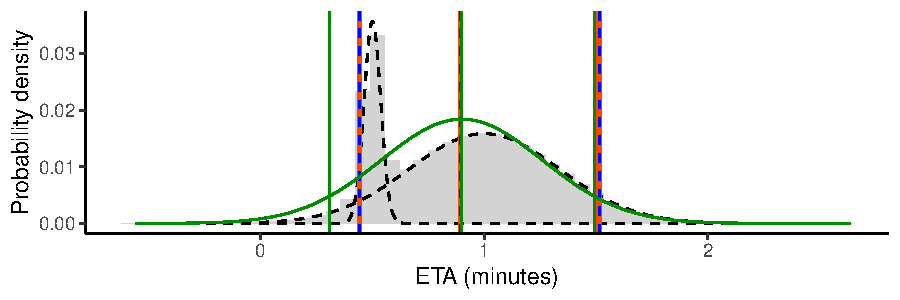
\includegraphics[width=\textwidth]{figure/normal_approx-1} 

}

\caption[Normal approximation for a series of stops ahead]{Normal approximation for a series of stops ahead. The true distribution is shown by the histogram with the underlying components (dashed curves). The vertical lines represent the quantiles computed using the sampled data, the normal mixture (using the optimisation formula), or a single normal approximation.}\label{fig:normal_approx}
\end{figure}


\end{knitrout}

A mixture of normal distributions can approximate the arrival time distribition \citep{Wang_2012} by expressing the mean and uncertainty as vectors $\tilde\mu$ and $\tilde\sigma^2$, respectively, along with a third vector $\tilde\pi$ denoting the $\tilde N$ mixture weights\footnote{We are using the tilde over parameters, e.g., $\tilde x$, to help distinguish them from others used throughout the thesis}, such that
\begin{equation}
\label{eq:ch5:mixture_weight_spec}
\tilde\pi_i > 0, i = 1, \ldots, \tilde N
\text{ and } \sum_{i=1}^{\tilde N} \tilde\pi_i = 1.
\end{equation}
The arrival time at stop $j + n$ is then given by
\begin{equation}
\label{eq:arrival_time_normal_approx}
\Tarr_{j+n} | \tilde\mu, \tilde\sigma^2, \tilde\pi, \RouteNWstate =
\sum_{\ell=j}^{j+n-1} \RouteNWstateseg_\ell +
\sum_{i=1}^{\tilde N} \tilde\pi_i z_i,\quad
z_i \sim \Normal{\tilde\mu_i}{\tilde\sigma^2_i}.
\end{equation}


Each component $i$ has an indicator $I_{im} = \{0,1\}$ of whether or not it stopped at stop $m$, so the total dwell time has mean and variance
\begin{equation}
\label{eq:mixture_dwell_times}
\tilde\mu_i = \sum_{m=j}^{j+n} I_{im} \dwell_m\quad\text{and}\quad
\tilde\sigma_i^2 = \sum_{m=j}^{j+n} I_{im} \dwellvar_m,
\end{equation}
respectively, assuming dwell times at individual stops are independent of each other.

Mixture weights are obtained through the stopping probability at each stop, $\pi_j$:
\begin{equation}
\label{eq:ch5:mixture_weights}
\tilde\pi_i = \prod_{m=j}^{j+n} \tilde p_{im}
\end{equation}
where
\begin{equation}
\label{eq:ch5:mixture_weights2}
\tilde p_{im} =
\begin{cases}
\pi_m & \text{if } I_{im} = 1 \\
1 - \pi_m & \text{otherwise.}
\end{cases}
\end{equation}


The mixture approximation works well for a few stops ahead, but after some time the mixture weights become small and the components combine, as shown in \cref{fig:normal_approx}. To prevent $\tilde N$ from becoming too large, the full distribution is simplified into a single component with mean and variance
\begin{equation}
\label{eq:mixture_mean}
\begin{split}
\E{\Tarr_m | \tilde\pi, \tilde\mu, \tilde\sigma^2, \RouteNWstate} &=
\E{\sum_{\ell=j}^{j+n-1} \RouteNWstateseg_\ell +
  \sum_{i=1}^{\tilde N} \tilde\pi_i z_i} \\
&= \sum_{\ell=j}^{j+n-1} \E{\RouteNWstateseg_\ell} +
  \sum_{i=1}^{\tilde N} \tilde\pi_i \E{z_i} \\
&= \sum_{\ell=j}^{j+n-1} \hat\RouteNWstateseg_\ell +
  \sum_{i=1}^{\tilde N} \tilde\pi_i \tilde\mu_i
\end{split}
\end{equation}
and
\begin{equation}
\label{eq:mixture_variance}
\begin{split}
\Var{\Tarr_m | \tilde\pi, \tilde\mu, \tilde\sigma^2, \RouteNWstate} &=
\Var{\sum_{\ell=j}^{j+n-1} \RouteNWstateseg_\ell +
  \sum_{i=1}^{\tilde N} \tilde\pi_i z_i} \\
&= \sum_{\ell=j}^{j+n-1} \Var{\RouteNWstateseg_\ell} +
  \sum_{i=1}^{\tilde N} \tilde\pi_i^2 \Var{z_i} \\
&= \sum_{\ell=j}^{j+n-1} \hat\RouteNWstatesegvar_\ell +
  \sum_{i=1}^{\tilde N} \tilde\pi_i \tilde\sigma_i^2
\end{split}
\end{equation}
respectively, assuming segment travel time and dwell time are independent---assuming otherwise makes this model impossible to work with; indeed, this model versus the particle filter (which makes no such assumption) is effectively testing the viability of this assumption.


An optimisation is used to obtain quantiles $q_\alpha$ such that
\begin{equation}
\label{eq:mixture_quadratic}
\left[
  p\left(\alpha \leq \Tarr_m | \tilde\pi, \tilde\mu, \tilde\sigma^2, \RouteNWstate\right) - q_\alpha
\right]^2 = 0.
\end{equation}
This is straightforward using Brent's Algorithm \citep{Brent_1971}, implemented in the Boost \textsf{C++} library.

When the 2.5\%, 50\%, and 97.5\% quantiles for the single approximation are within 30~seconds of the same quantiles computed for the mixture distribution, the mixture is replaced with one single component with mean and variance defined in \cref{eq:mixture_mean,eq:mixture_variance}. In some situations, the mixture may not converge into a single distribution quick enough, so to prevent the number of components $\tilde N$ from exceeding $2^8=256$, all components with weights less than a predefined threshold (we used $\frac{1}{2}\max_i(\pi_i)$) are combined into a single component.
